\documentclass[11pt]{article}

\usepackage[utf8]{inputenc}

\usepackage{amsmath, bm}
\usepackage{graphicx}
\usepackage{amssymb}
\usepackage{float}
\usepackage{caption}
\usepackage{subcaption}
\usepackage{hyperref}
\usepackage{tikz}
\usepackage{layout}
\usepackage{wrapfig}

\usepackage[margin=1in]{geometry}
\usepackage{listings}
\usepackage{xcolor}
\usepackage{color, colortbl}
\usepackage{textgreek}
\usepackage{mathrsfs}
\usepackage{savetrees}

% 12 pt font
\renewcommand{\normalsize}{\fontsize{12pt}{\baselineskip}\selectfont}

\begin{document}

\title{4A7 Transonic Wing Design}
\author{lwp26}
\date{May 2024}
\maketitle

\section{Introduction}


The development of high-efficiency aerofoils, can significantly improve the overall performance of an aircraft.
The Breguet range equation, which calculates the range of an aircraft, directly depends on the flight speed and lift to drag ratio of the wing:

\begin{equation}
S = \frac{U}{g}\frac{L/D}{\text{sfc}} \log \left( \frac{W_\text{start}}{W_\text{end}} \right)
\end{equation}

where $S$ is the range, $U$ is the flight velocity, $g$ is the acceleration due to gravity, $\text{sfc}$ is the specific fuel consumption of the engine, and $W_\text{start}$ and $W_\text{end}$ are the initial and final weights of the aircraft, respectively.
This shows increasing flight speed and lift to drag ratio will increase the range of the aircraft.
In the troposphere where temperature decreases, maximising range is equivalent to maximising $M \cdot L/D$.

Previous work in subsonic airfoil design maximising $L/D$ showed the importance of the boundary layer growth on the viscous drag of the wing.
Adjustments were made to surface curvature, changing pressure gradients in effort to delay transition and separation, minimising boundary layer growth \cite{SA1_report}.
Transonic airfoil design is more complex than subsonic design due to the formation of shock waves on the wing surface.
Additional lift is obtained by maximising suction peak and area of supersonic flow, however there is an additional source of wave drag that increases with shock strength.
The general goal of our design process therefore was to delay the position and strength of the shock wave.
However, this location and strength were observed to be highly sensitive to the geometry, which is likely due to small changes to Prantle Meyer
expansion fan angles causing large changes in the position of reflected compression lines from the constant pressure boundary.
These expansion angles are also dependent on local geometry and local Mach number, causing a chaotic design space.
 
\section{Design Process}

High curvature at the leading edge provides rapid expansion to the suction peak, maximising lift here.
The first spline point had to be moved down to ensure ther was no inflection point on the upper surface due to centerline spline and thickness distribution.
A very small amount of curvature is maintained around the top surface to prevent further expansion in the supersonic region,
and to allow the reflected expansion lines to compress the flow, reducing the shock strength.
Flatter and concave curvatures at mid-chord of the upper surface were tested but these increased curvature at the trailing edge, increasing back pressure which caused two shocks to form.
This region of increased curvature is required to return to the surface back to the trailing edge.
At the end of the upper surface, there is some concave geometry where the upper and lower pressure distributions cross over.
This causes downforce, which is poor for lift and comes as a result of the thickness distribution.

\section{Limitations}

The software is only valid for 2D infinite length wings. This neglects the effects of downwash due to wing tip vortices and other 3D flow effects.
VGK also relies on the Lag-Entrainment integral method for turbulent boundary layers which relies on empirical correlations
and poorly models some shock boundary layer interactions \cite{lagentrainment}.
Numerical errors can also arise from the discretisation of the geometry and the flow field.
Cases where the VGK software fails to converge are not included in the data set and the cause of these failures may be unsteady buffeting or general impractical flow conditions.
A personal hypothesis is having control over both upper and lower surface splines, rather than a thickness distribution, could improve the design process.
While this may increase the dimensionality of the problem, it reduces ill-conditioning and coupled effects.

% reference SA1 wing analysis report

\begin{figure}
    \centering
    \begin{subfigure}[t]{0.48\textwidth}
        \centering
        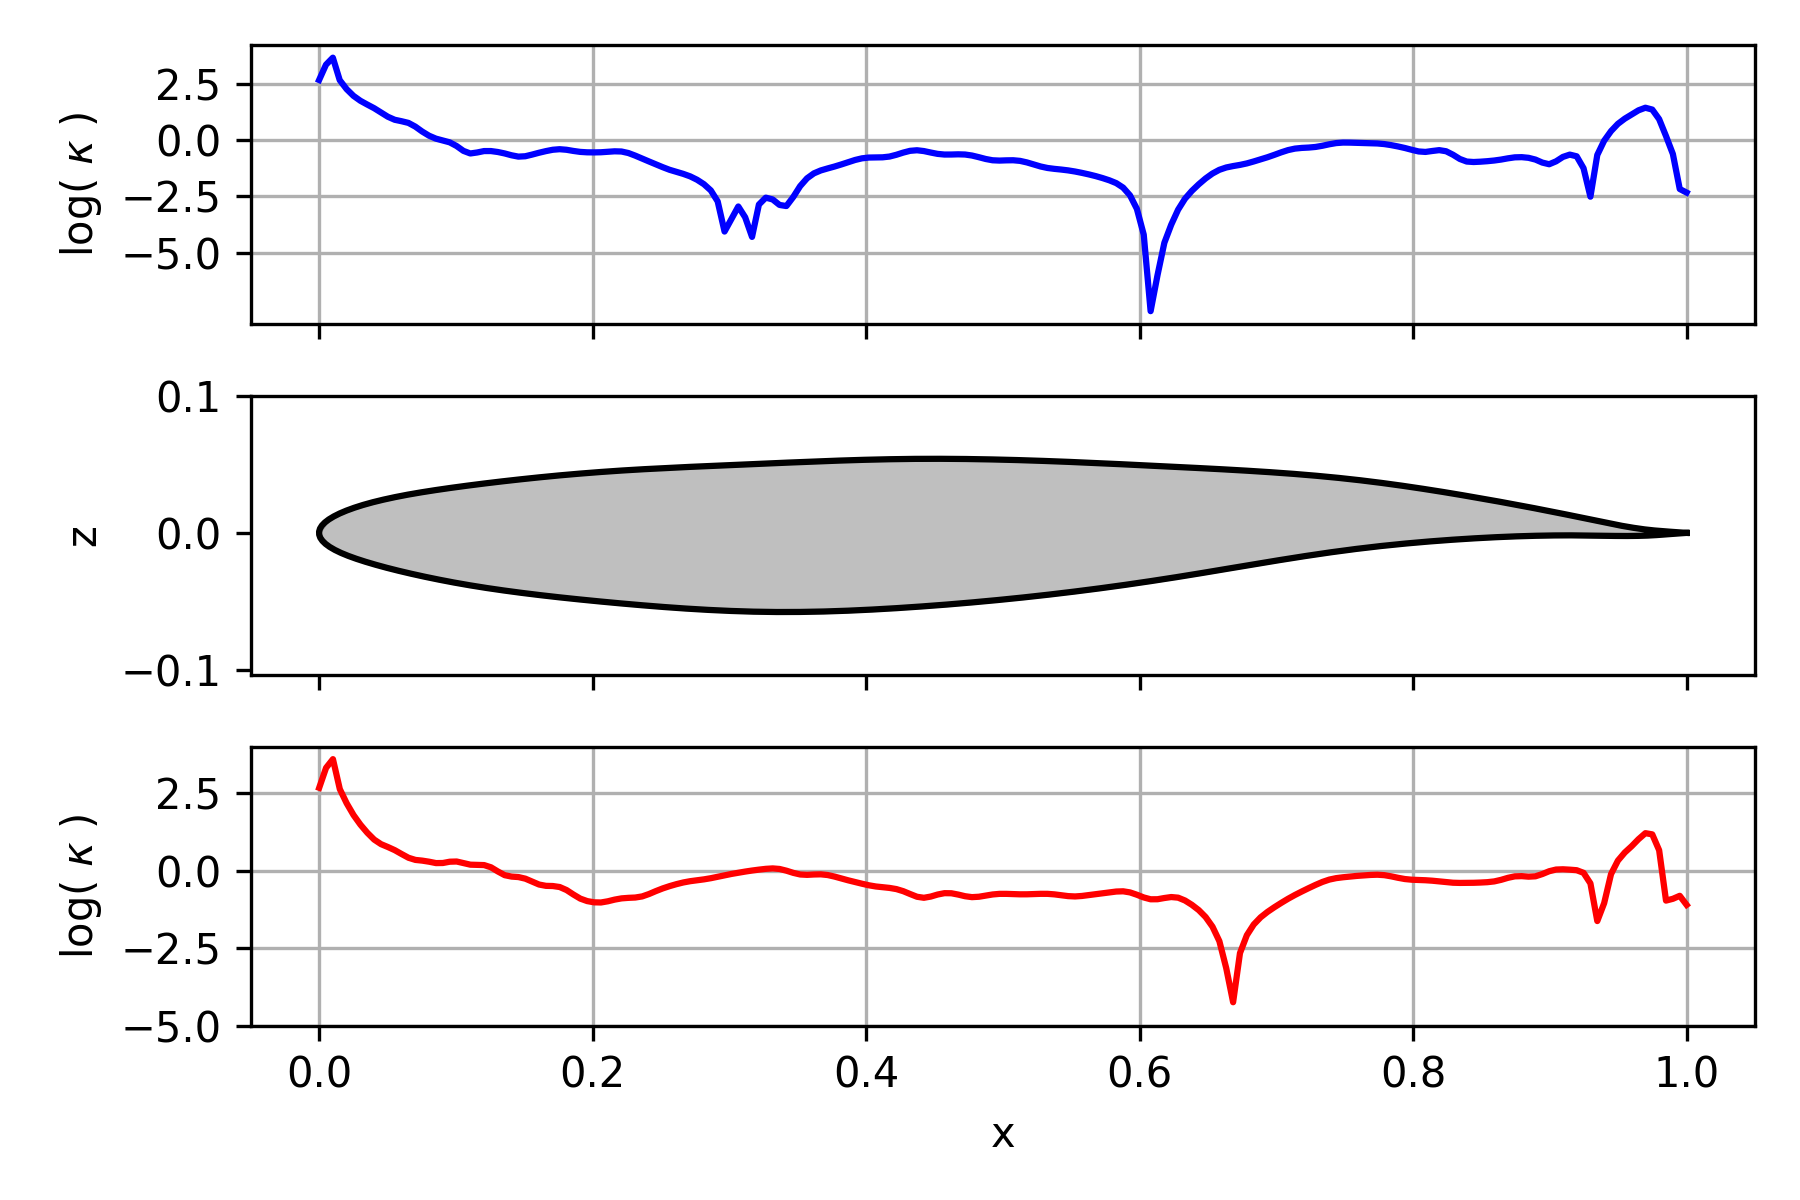
\includegraphics[width=\textwidth]{figures/airfoil.png}
        \caption{Aerofoil cross-section}
        \label{fig:airfoil}
    \end{subfigure}
    \begin{subfigure}[t]{0.48\textwidth}
        \centering
        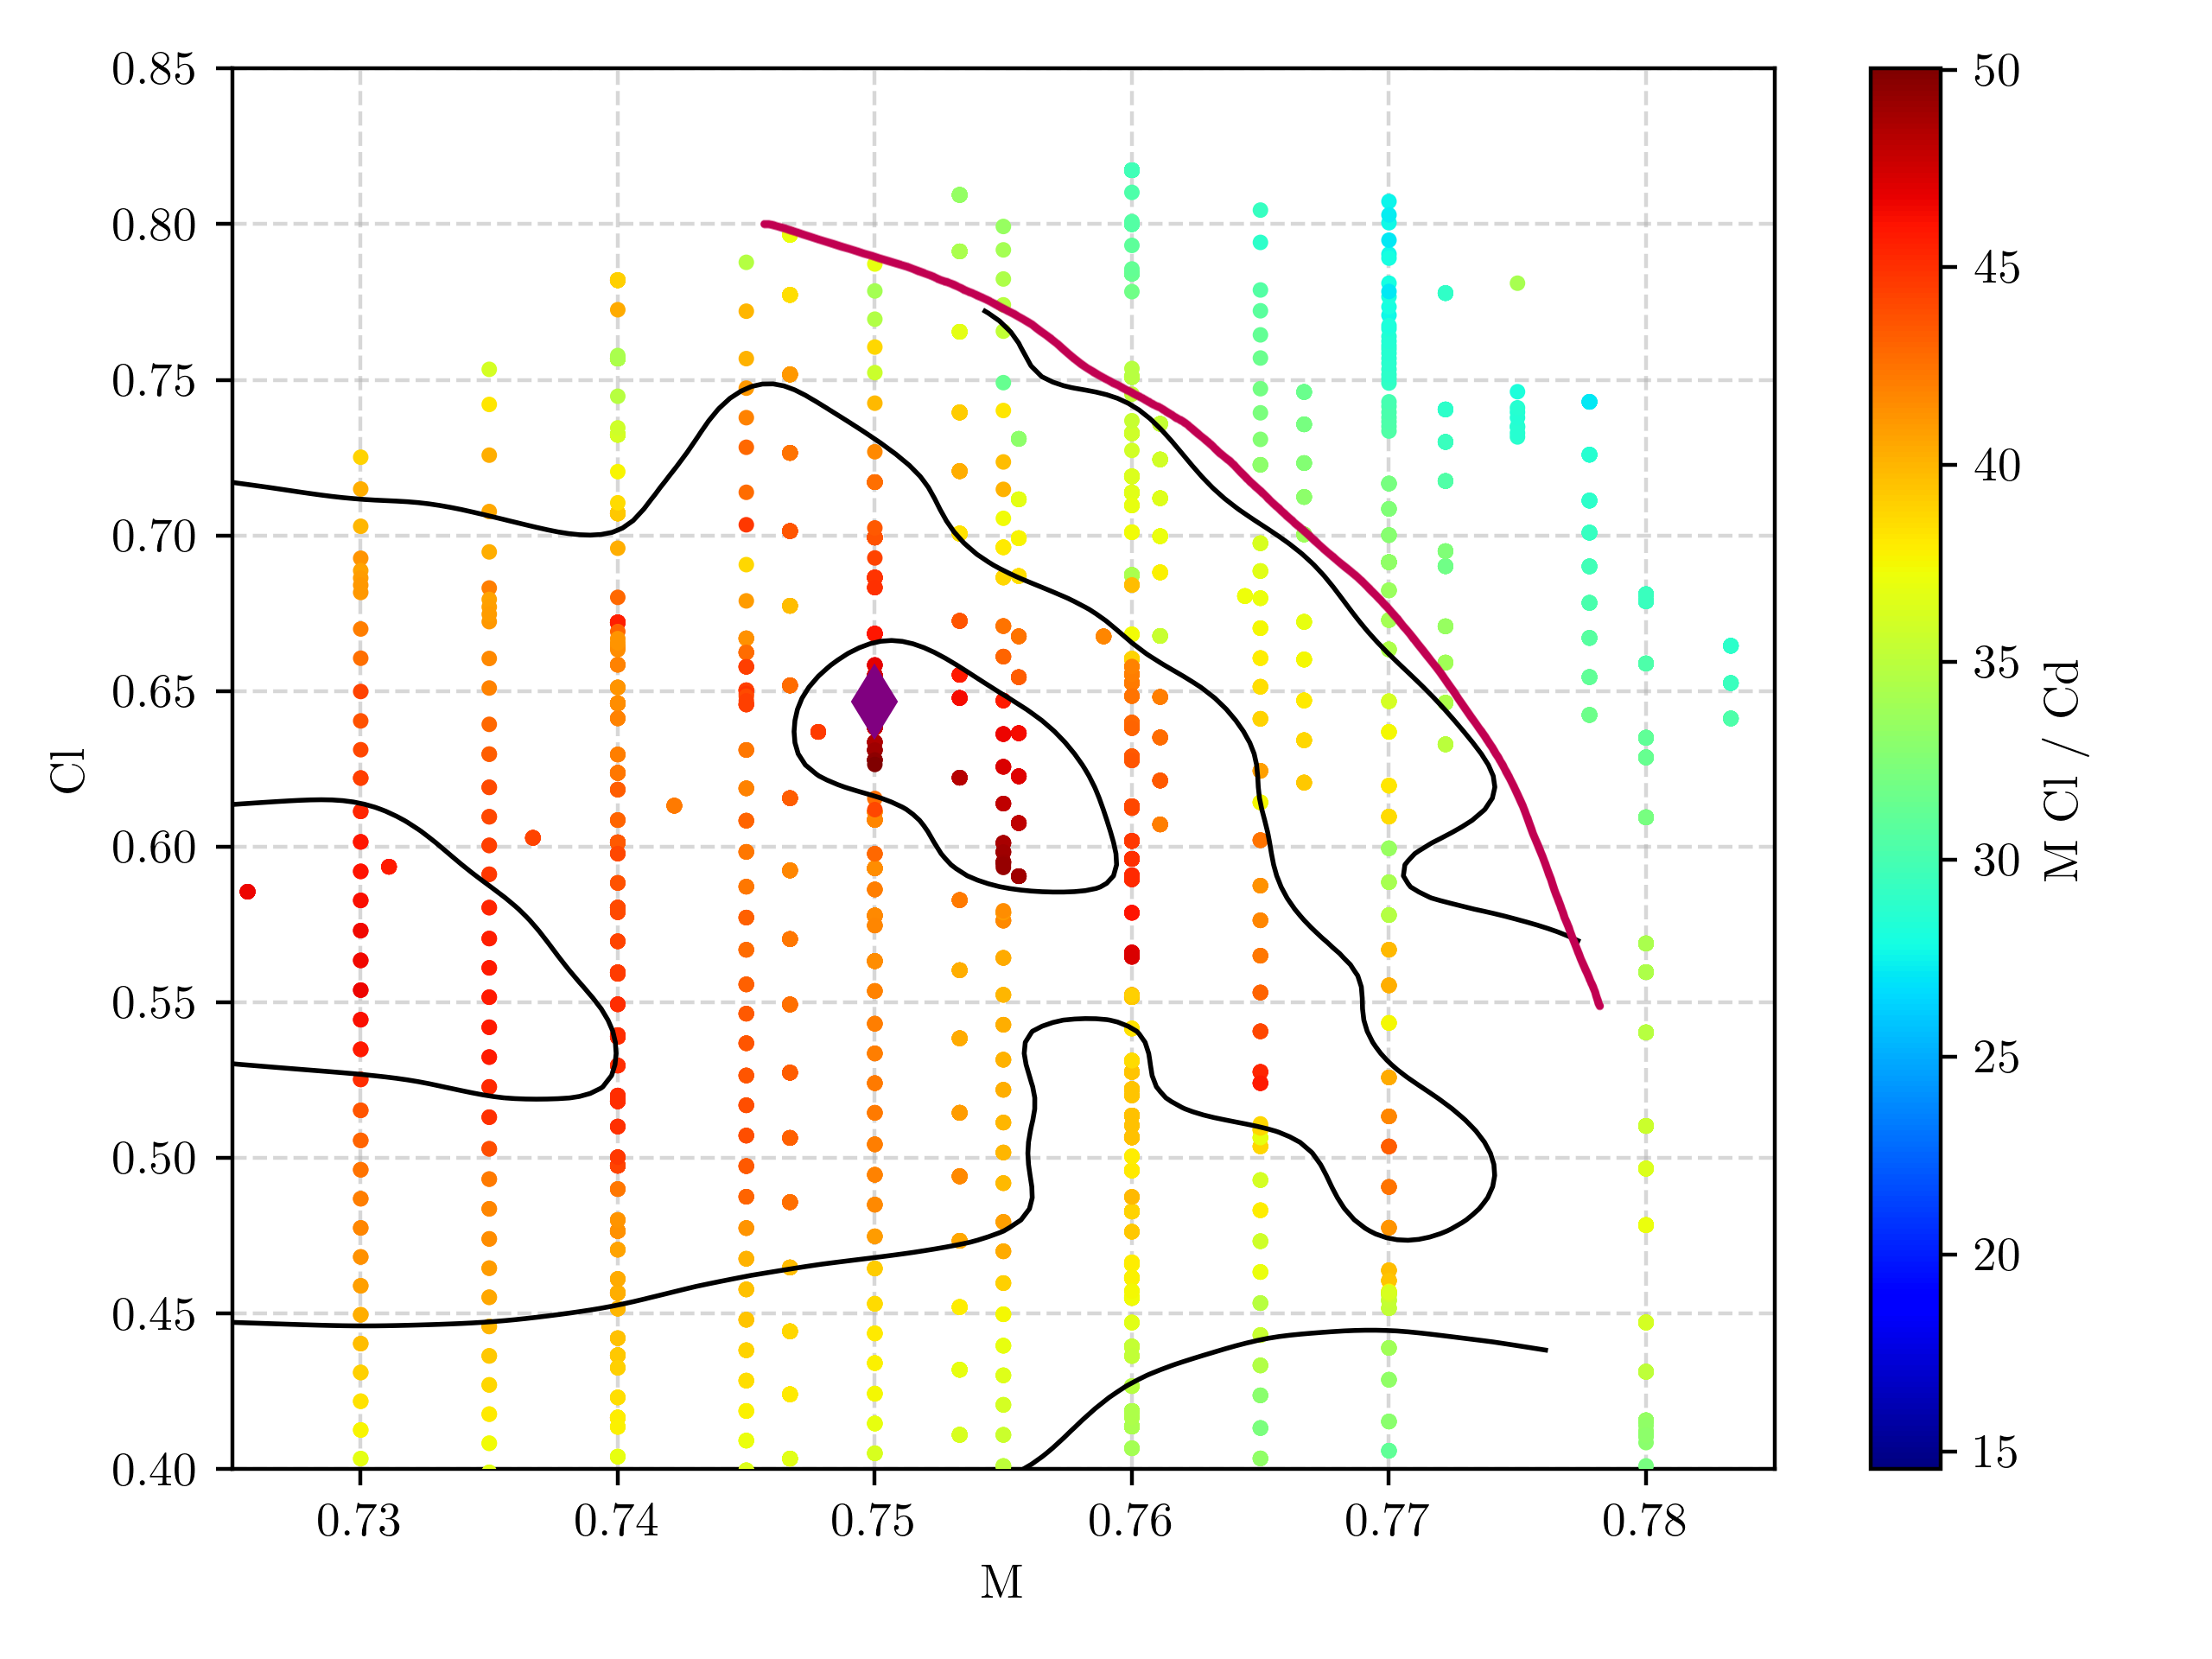
\includegraphics[width=0.9\textwidth]{figures/performance_metric.png}
        \caption{Performance metric and drawn buffet line}
        \label{fig:performance_metric}
    \end{subfigure}
    \caption{}
\end{figure}


\begin{figure}
    \centering
    \begin{subfigure}[t]{0.45\textwidth}
        \centering
        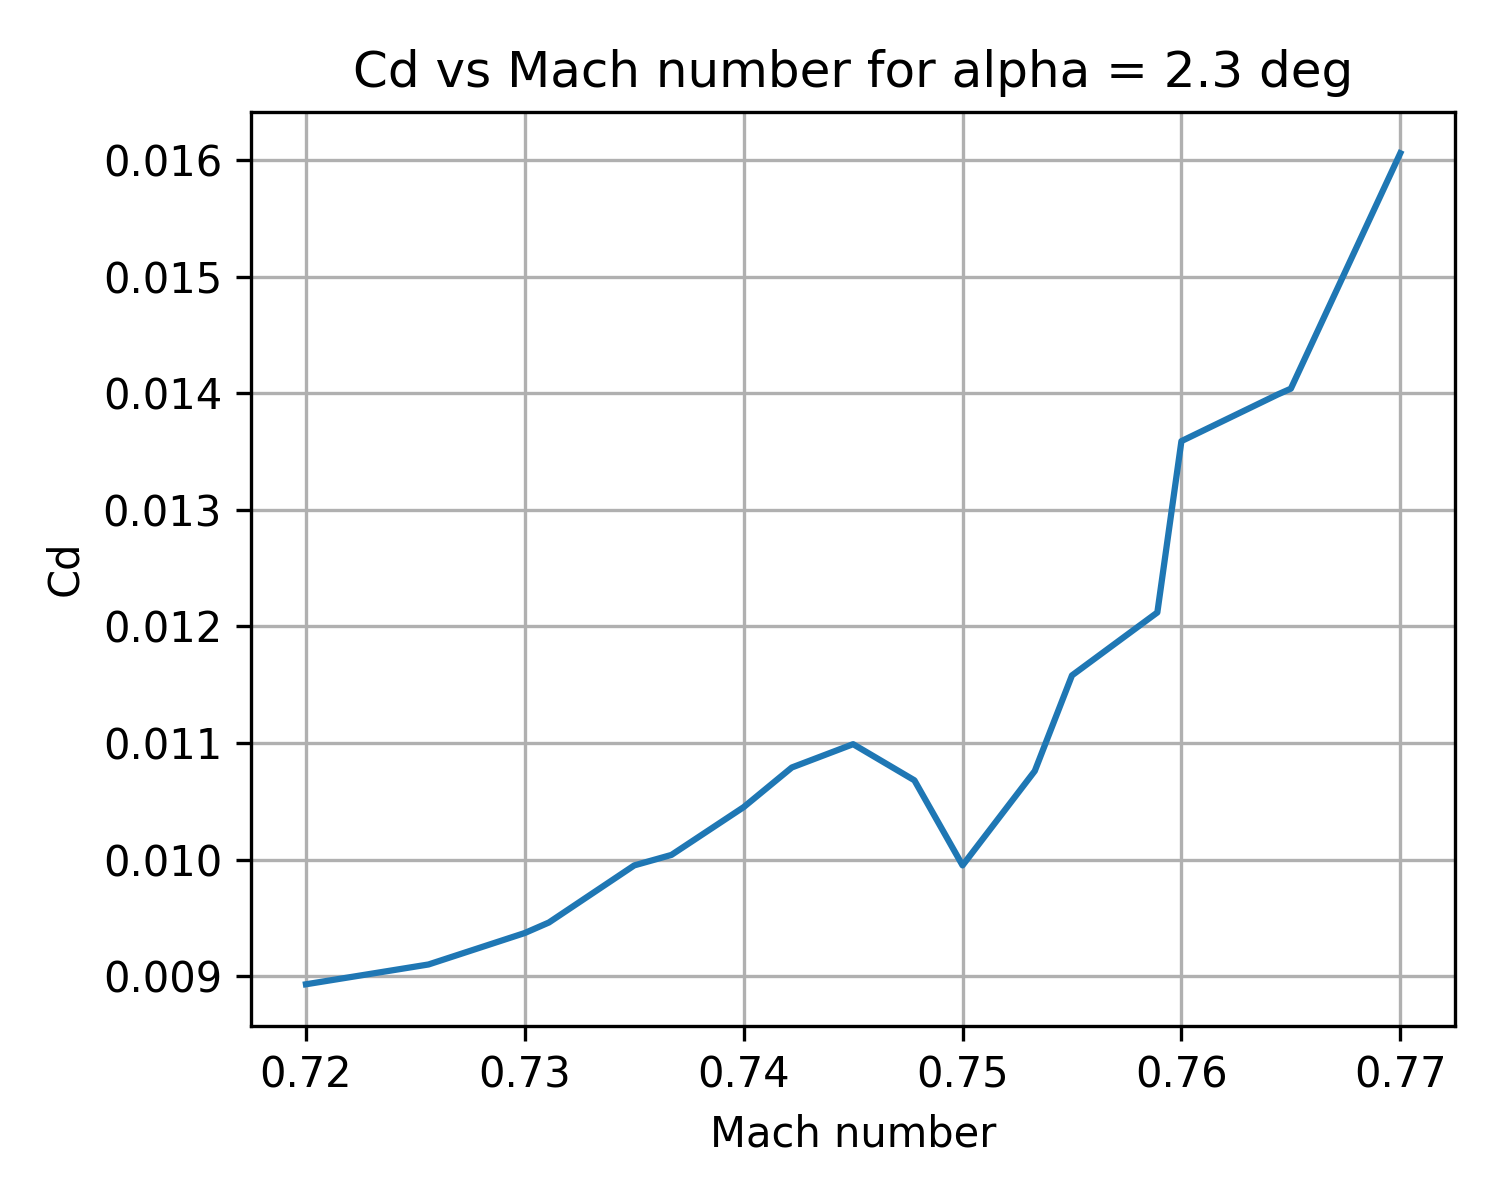
\includegraphics[width=\textwidth]{figures/cd_vs_mach.png}
        \caption{Drag coefficient vs Mach number}
        \label{fig:cd_vs_mach}
    \end{subfigure}
    \begin{subfigure}[t]{0.45\textwidth}
        \centering
        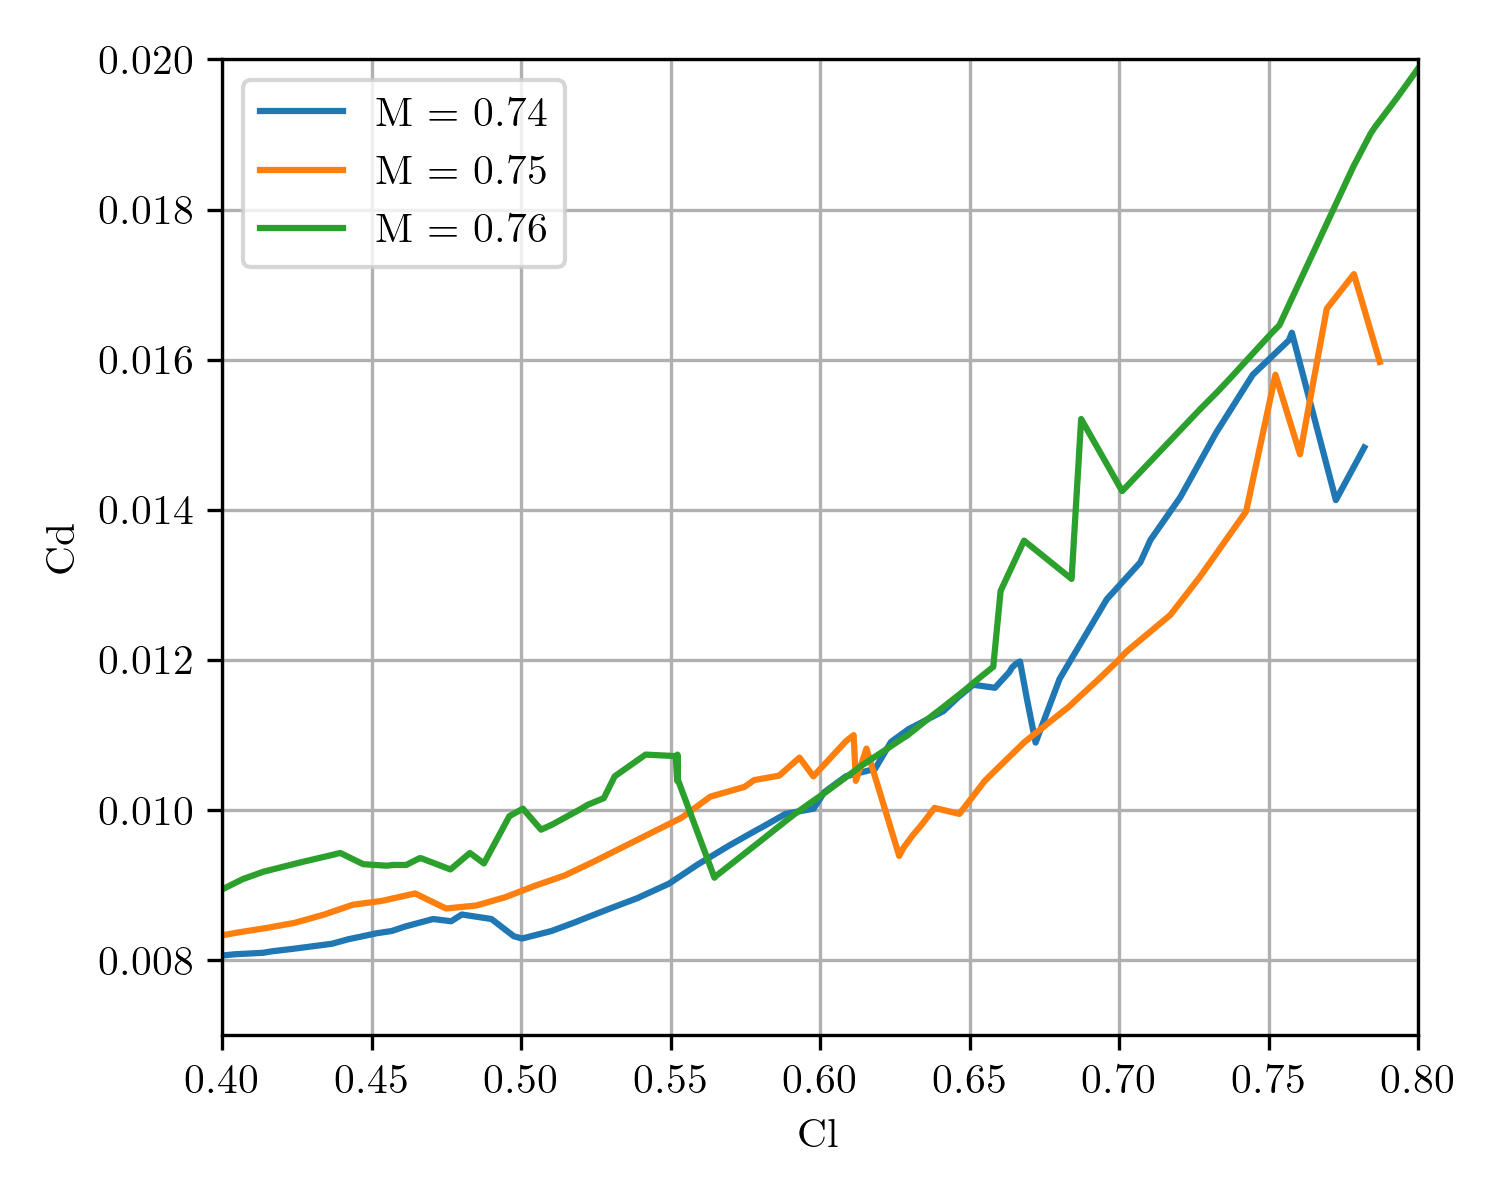
\includegraphics[width=\textwidth]{figures/cd_vs_cl.png}
        \caption{Pressure coefficient distribution for different Mach numbers}
        \label{fig:cd_vs_cl}
    \end{subfigure}
\end{figure}


\section{Buffet Line}

Buffet is complex unstable interaction between the shockwaves and boundary layers and can produce large amplitude pressure fluctuations on the wing surface.
This can be damaging to the aircraft structure and cause a loss of control.

There are various measures to detect the onset of buffet
\begin{itemize}
    \item Shock entry Mach number, taken at shock of maximum strength
    \item Trailing edge shape factor, $\overline{H}_{te}$
    \item High Mach numbers close to trailing edge, measured by a minimum distance between Mach distribution and line $M_{lin}$.
    \item Trailing edge pressure coefficient rise of 0.04 above its plateau value.
\end{itemize}
These are quantified in the non-dimensional buffet factors, seen on Figure \ref{fig:buffet_classification}.
The data consists of 4684 converged solutions at different Mach numbers and angles of attack which were automatically collected using a Python script.
The first factor is a first indication that the shock is strong enough to cause buffet.
This shows that in many operating points of high Mach number and lift coefficient, the shock is strong enough to cause buffet.

The second factor indicates trailing edge separation, which is a necessary condition for buffet.

\begin{figure}
    \centering
    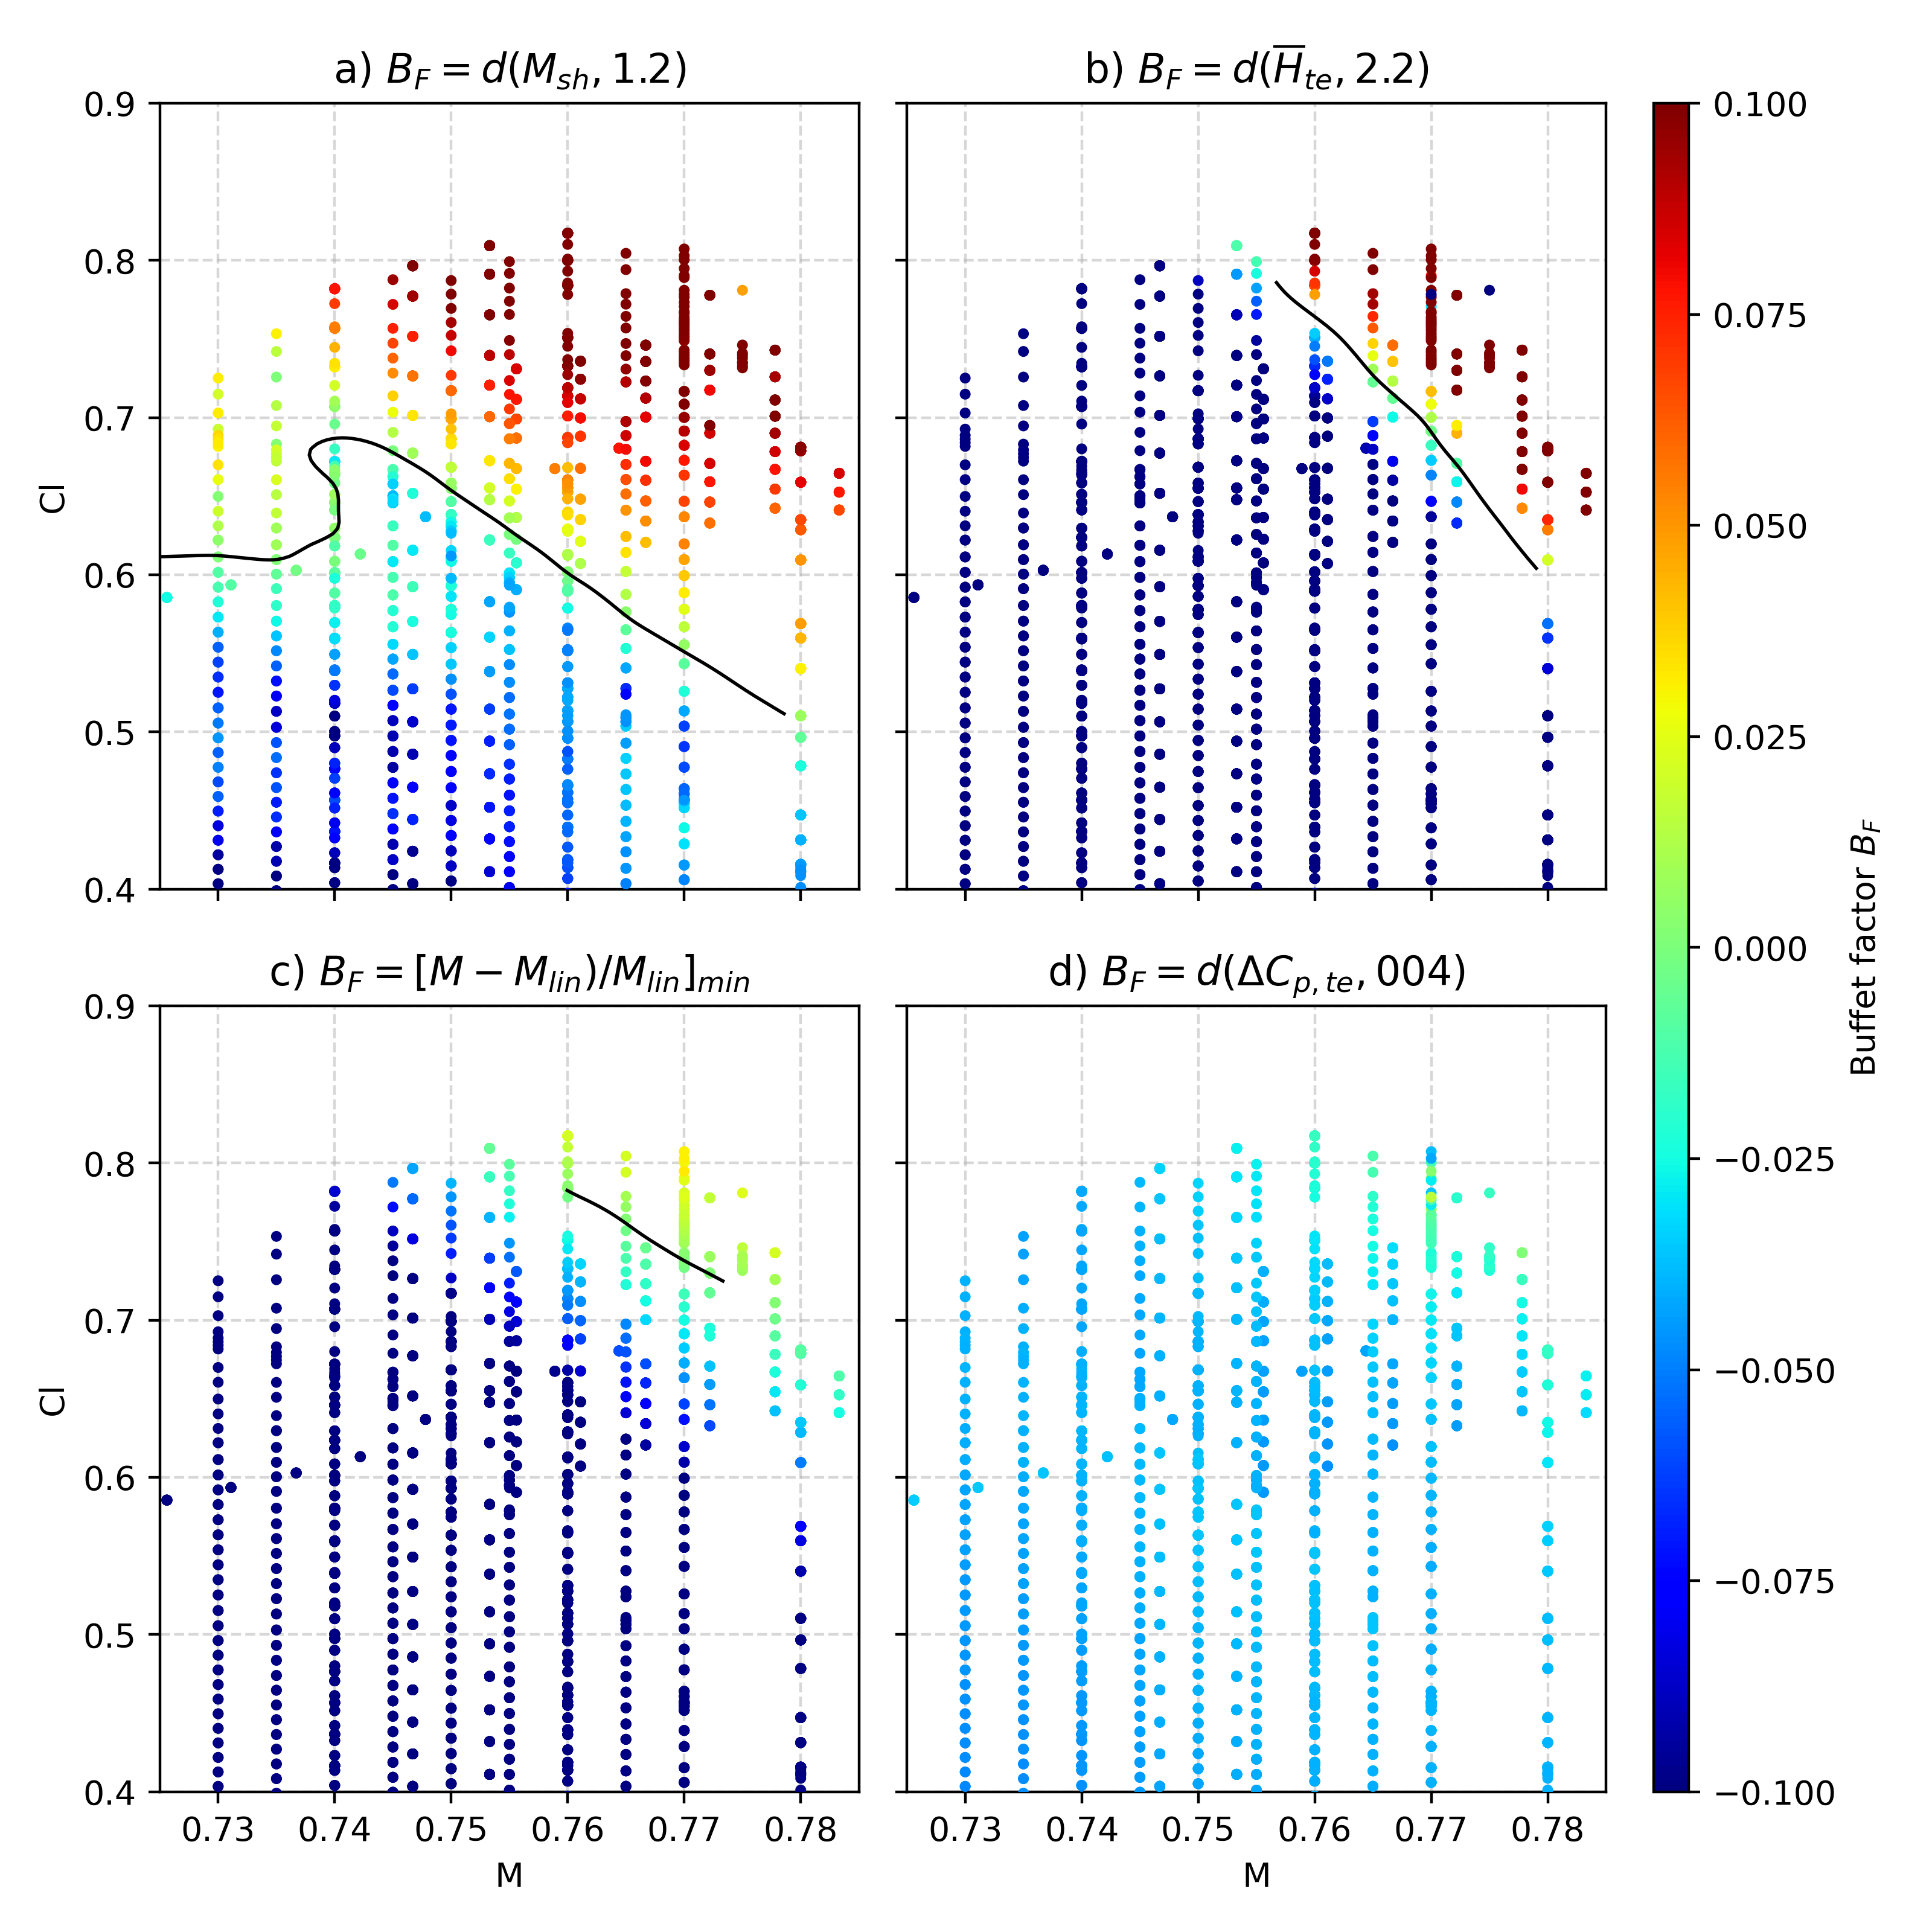
\includegraphics[width=0.8\textwidth]{figures/buffet_classification.png}
    \caption{Buffet factors at a range of Mach numbers and lift coefficients. $d(x,c)$ is the normalised difference $(x-c)/c$}
    \label{fig:buffet_classification}
\end{figure}

\begin{thebibliography}{9}


      \bibitem{SA1_report}
      L. W. Pender
      \emph{SA1 Wing Analysis Final Report}
      University of Cambridge,
      2024.
    
      \bibitem{handout}
      J. Jarret
      \emph{4A7 Transonic Wing Design Handout}
      University of Cambridge,
      2024.

        \bibitem{lagentrainment}
        Green J E, Weeks D J and Brooman J W F,
        \emph{Prediction of turbulent boundary-layers and wakes in compressible flow by a lag-entrainment method.}
        ARC
    
\end{thebibliography}

\end{document}